% !TEX root = 02.tex

\section{Analysis Passes}
\begin{frame}{Checking Input Properties}
Analysis basically allows to:
\begin{itemize}
\item \alert{derive} information and properties of the input
\item \alert{verify} properties of input
\end{itemize}

\vfill
Keeping analysis information is expensive:
\begin{itemize}
\item tuned algorithms updates analysis information when an optimization
      invalidates them
\item incrementally updating analysis is cheaper than recomputing them
\end{itemize}

\vfill
Many LLVM analysis supports incremental updates:
\begin{itemize}
\item this is an \alert{optimization}
\item focus on \alert{information} provided by analysis
\end{itemize}
\end{frame}

\begin{frame}{Useful Analysis}
We will see the following passes:

\begin{block}{Analysis}
\centering
\begin{tabular}{ccc}
\toprule

\multicolumn{1}{c}{\textbf{Pass}}        &
\multicolumn{1}{c}{\textbf{Switch}}      &
\multicolumn{1}{c}{\textbf{Transitive}} \\

\midrule

Control flow graph  &
\texttt{none}       &
No                 \\

Dominator tree    &
\texttt{domtree}  &
No               \\

Post-dominator tree   &
\texttt{postdomtree}  &
No                   \\

Loop information  &
\texttt{loops}    &
Yes              \\

Scalar evolution           &
\texttt{scalar-evolution}  &
Yes                       \\

Alias analysis    &
\texttt{special}  &
Yes              \\

Memory dependence  &
\texttt{memdep}    &
Yes               \\

\bottomrule
\end{tabular}
\end{block}
\end{frame}

\begin{frame}{Require Analysis}
Ask the pass manager to schedule a specific pass
before running the current one.

\vfill
Requiring analysis by transitivity:
\begin{description}
\item[yes] \cppinline{llvm::AnalysisUsage::addRequiredTransitive<T>()}
\item[no] \cppinline{llvm::AnalysisUsage::addRequired<T>()}
\end{description}

\vfill
In cases where \alert{analyses chain},the addRequiredTransitive method
should be used instead of the addRequired method.

This informs the PassManager that the transitively required pass
should be alive as long as the requiring pass is.
\end{frame}

\begin{frame}{Control Flow Graph}
The Control Flow Graph is implicitly maintained by LLVM:

\begin{itemize}
\item no specific pass to build it
\end{itemize}

\vfill
Recap:

\begin{itemize}
\item CFG for a function is a set of basic blocks
\item a basic block is a set of instructions
\end{itemize}

\vfill
Functions and basic blocks acts like containers:

\begin{itemize}
\item STL-like accessors: \cppinline{front()}, \cppinline{back()},
      \cppinline{size()}, \ldots
\item STL-like iterators: \cppinline{begin()}, \cppinline{end()}
\end{itemize}

\vfill
Each contained element is aware of its container:

\begin{itemize}
\item \cppinline{getParent()}
\end{itemize}
\end{frame}

\begin{frame}{Control Flow Graph}{Walking}
Every CFG has an entry basic block:

\begin{itemize}
\item the \alert{first} executed basic block
\item it is the \alert{root/source} of the graph
\item get it with \cppinline{llvm::Function::getEntryBlock()}
\end{itemize}

\vfill
More than one exit blocks can be generated:

\begin{itemize}
\item their terminator instructions are \llvminline{ret}s
\item they are the \alert{leaves/sinks} of the graph
\item use \cppinline{llvm::BasicBlock::getTerminator()} to get the terminator
      \ldots
\item \ldots then check its real class
\end{itemize}
\end{frame}

\begin{frame}{Side Note}{Casting Framework}
For performance reasons, a custom casting framework is used:

\begin{itemize}
\item you cannot use \cppinline{static\_cast} and \cppinline{dynamic\_cast} with
      types/classes provided by LLVM
\end{itemize}

\begin{block}{LLVM Casting Functions}
\centering
\begin{tabular}{cc}
\toprule

\multicolumn{1}{c}{\textbf{Meaning}}   &
\multicolumn{1}{c}{\textbf{Function}} \\

\midrule

Static cast of \cppinline{Y *} to \cppinline{X *}  &
\cppinline{X * llvm::cast<X>(Y *)}                \\

Dynamic cast of \cppinline{Y *} to \cppinline{X *}  &
\cppinline{X * llvm::dyn\_cast<X>(Y *)}            \\

Is \cppinline{Y} an \cppinline{X}?  &
\cppinline{bool llvm::isa<X>(Y *)} \\

\bottomrule
\end{tabular}
\end{block}

Example:

\begin{itemize}
\item is \cppinline{BB} a sink?
      \begin{center}
      \cppinline{llvm::isa<llvm::ReturnInst>(BB.getTerminator())}
      \end{center}
\end{itemize}
\end{frame}

\begin{frame}{Control Flow Graph}{Basic Blocks}
Every basic block \cppinline{BB} has one or more:

\begin{description}
\item[predecessors] from \cppinline{pred\_begin(BB)} to
      \cppinline{pred\_end(BB)} \footnote{see include/llvm/IR/CFG.h}
\item[successors] from \cppinline{succ\_begin(BB)} to
      \cppinline{succ\_end(BB)}
\end{description}

\vfill
Convenience accessors directly available in \cppinline{llvm::BasicBlock}:

\begin{itemize}
\item e.g. \cppinline{llvm::BasicBlock::getUniquePredecessor()}
\end{itemize}

Other convenience member functions:

\begin{itemize}
\item moving a basic block:
      \cppinline{llvm::BasicBlock::moveBefore(llvm::BasicBlock *)} or
      \cppinline{llvm::BasicBlock::moveAfter(llvm::BasicBlock *)}
\item split a basic block:
      \cppinline{llvm::BasicBlock::splitBasicBlock(llvm::BasicBlock::iterator)}
\item \ldots
\end{itemize}
\end{frame}

\begin{frame}{Control Flow Graph}{Instructions}
The \cppinline{llvm::Instruction} class define common operations:

\begin{itemize}
\item e.g. getting an operand: \cppinline{llvm::Instruction::getOperand(unsigned)}
\end{itemize}

Subclasses provide specialized accessors:

\begin{itemize}
\item e.g the \llvminline{load} instruction takes an operand that is a pointer:
      \cppinline{llvm::LoadInst::getPointerOperand()}
\end{itemize}

\pause
\vfill
The value produced by the instruction is the \alert{instruction itself}:

\begin{block}{Example}
Consider:

\centering
\llvminline{\%6 = load i32, i32* \%1, align 4}

\flushleft
the \llvminline{load} is described
by an instance of \cppinline{llvm::LoadInst}. That instance also models the
\llvminline{\%6} variable
\end{block}
\end{frame}

\begin{frame}{Instructions}{Creating New Instructions}
Instructions built using:

\begin{itemize}
\item constructors -- e.g. \cppinline{llvm::LoadInst::LoadInst(...)}
\item factory methods -- e.g. \cppinline{llvm::GetElementPtrInst::Create(...)}
\end{itemize}

Interface is not homogeneous:

\begin{itemize}
\item some instructions support both methods
\item others support only one
\end{itemize}

\vfill
At build-time, instructions can be:

\begin{itemize}
\item appended to a basic block
\item inserted after/before a given instruction
\end{itemize}

Insertion point usually specified as builder last argument
\end{frame}

\begin{frame}{Side Note}{Definitions and Uses}
LLVM class hierarchy is built around two simple concepts:

\begin{description}
\item[value] something that can be used: \cppinline{llvm::Value}
\item[user] something that can use: \cppinline{llvm::User}
\end{description}

A value is a \alert{definition}:

\begin{itemize}
\item \cppinline{llvm::Value::use\_begin()},
      \cppinline{llvm::Value::use\_end()} to visit uses
      \footnote{\cppinline{llvm::Instruction} derives from \cppinline{llvm::Value}}
\end{itemize}

An user access \alert{definitions}:

\begin{itemize}
\item \cppinline{llvm::User::op\_begin()},
      \cppinline{llvm::User::op\_end()} to visit used values
      \footnote{\cppinline{llvm::Value} derives from \cppinline{llvm::User}}
\end{itemize}

\vfill
\begin{columns}[t]
\column{.45\textwidth}
Functions:

\begin{itemize}
\item used by call sites
\item uses formal parameters
\end{itemize}

\column{.45\textwidth}
Instructions:

\begin{itemize}
\item define an SSA value
\item uses operands
\end{itemize}
\end{columns}
\end{frame}

\begin{frame}{Side Note}{Value Typing}
Every \cppinline{llvm::Value} is typed:

\begin{itemize}
\item use \cppinline{llvm::Value::getType()} to get the type
\end{itemize}

\vfill
Since every instructions is/define a value:

\begin{itemize}
\item instructions are typed
\end{itemize}

\vfill
\begin{block}{Example}
Consider:

\centering
\llvminline{\%6 = load i32, i32* \%1, align 4}

\flushleft
\begin{itemize}
\item The \llvminline{\%6} variable actually is the instruction itself
\item Its type is the type of \llvminline{load} return value, \llvminline{i32}
\end{itemize}
\end{block}
\end{frame}

\begin{frame}{Dominance Trees}
Dominance trees answer to control-related queries:

\begin{columns}[t]
\column{.45\textwidth}
\begin{itemize}
\item is this basic block executed before that?
\item \cppinline{llvm::DominatorTree}
\end{itemize}

\column{.45\textwidth}
\begin{itemize}
\item is this basic block executed after that?
\item \cppinline{llvm::PostDominatorTree}
\end{itemize}
\end{columns}

\vfill
The two trees interface is similar:

\begin{itemize}
\item \cppinline{bool dominates(X *, X *)}
\item \cppinline{bool properlyDominates(X *, X *)}
\end{itemize}

Where \cppinline{X} is an \cppinline{llvm::BasicBlock} or an
\cppinline{llvm::Instruction}

\vfill
by using \texttt{opt}, it is possible print them:

\begin{itemize}
\item \texttt{-view-dom}, \texttt{-dot-dom}
\item \texttt{-view-postdom}, \texttt{-dot-postdom}
\end{itemize}
\end{frame}

\begin{frame}{Loop Information}
Loop information are represented using two classes:

\begin{itemize}
\item \cppinline{llvm::LoopInfo} analysis detects natural loops
\item \cppinline{llvm::Loop} represents a single loop
\end{itemize}

\vfill
Using \cppinline{llvm::LoopInfo} it is possible:

\begin{itemize}
\item navigate through top-level loops: \\
      \cppinline{llvm::LoopInfo::begin()}, \cppinline{llvm::LoopInfo::end()}
\item get the loop for a given basic block: \\
      \cppinline{llvm::LoopInfo::operator[](llvm::BasicBlock *)}
\end{itemize}
\end{frame}

\begin{frame}{Loop Information}{Nesting Tree}
Loops are represented in a \alert{nesting tree}:

\begin{columns}[t]
\column{.45\textwidth}
\begin{block}{Source}
\centering
\cinput{snippet/loop-nest.c}
\end{block}

\column{.45\textwidth}
\begin{block}{Loop Nest}
\centering

% loop-nest.tex: a simple loop nest.

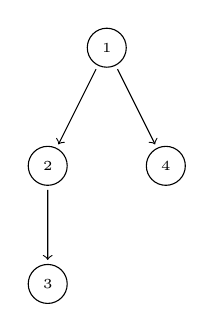
\begin{tikzpicture}
[
  every node/.style={
    font=\tiny
  },
  loop/.style={
    circle,
    draw
  },
  tip/.style={
    shorten <=.5mm,
    shorten >=.5mm,
    ->,
    draw
  },
  level 1/.style={
    edge from parent/.style=tip
  },
]

\node [loop] {$1$}
  child { node [loop] {$2$}
    child { node [loop] {$3$}}
  }
  child { node [loop] {$4$}};
\end{tikzpicture}

\end{block}
\end{columns}

Nest navigation:

\begin{itemize}
\item children loops: \cppinline{llvm::Loop::begin()},
      \cppinline{llvm::Loop::end()}
\item parent loop: \cppinline{llvm::Loop::getParentLoop()}
\end{itemize}
\end{frame}

\begin{frame}{Loop Information}{Query Loops}
Accessors for relevant nodes also available:

\begin{description}
\item[pre-header] \cppinline{llvm::Loop::getLoopPreheader()}
\item[header] \cppinline{llvm::Loop::getHeader()}
\item[latch] \cppinline{llvm::Loop::getLoopLatch()}
\item[exiting] \cppinline{llvm::Loop::getExitingBlock()}, \\
               \cppinline{llvm::Loop::getExitingBlocks(...)}
\item[exit] \cppinline{llvm::Loop::getExitBlock()} \\
            \cppinline{llvm::Loop::getExitBlocks(...)}
\end{description}

\vfill
Loop basic blocks accessible via:

\begin{description}
\item[iterators] \cppinline{llvm::Loop::block\_begin()}, \\
                 \cppinline{llvm::Loop::block\_end()}
\item[vector]
      \cppinline{std::vector<llvm::BasicBlock *> \&llvm::Loop::getBlocks()}
\end{description}
\end{frame}


\begin{frame}{Scalar Evolution}
The \alert{SC}alar \alert{EV}olution framework:

\begin{itemize}
\item represents scalar expressions
\item supports recursive updates
\item lower burden of explicitly handling expressions composition
\item is designed to support \alert{general induction variables}
\end{itemize}

\vfill
\begin{columns}\column{.64\textwidth}
\begin{block}{Example}
\centering
\llvminput{snippet/basic-scev.ll}
\end{block}

\column{.30\textwidth}
SCEV for \llvminline{\%i.0}:

\begin{itemize}
\item initial value $0$
\item incremented
\item by $1$ at each iteration
\item final value $10$
\end{itemize}
\end{columns}
\end{frame}

\begin{frame}{Scalar Evolution}{Example}
\begin{columns}
\column{.55\textwidth}
\begin{block}{Source}
\centering
\cinput{snippet/nested-scev.c}
\end{block}

\column{.35\textwidth}
SCEV \llvminline{\{A,B,C\}<\%D>}:

\begin{itemize}
\item \llvminline{A} initial
\item \llvminline{B} operator
\item \llvminline{C} operand
\item \llvminline{D} defining BB
\end{itemize}
\end{columns}

\vfill
\begin{block}{Induction Variables}
\centering
\llvminput{snippet/nested-scev-induction.ll}
\end{block}
\end{frame}

\begin{frame}{Scalar Evolution}{More than Induction Variables}
The scalar evolution framework manages \alert{any scalar expression}:

\begin{block}{Pointer SCEVs}
\centering
\llvminput{snippet/nested-scev-pointer.ll}
\end{block}

\vfill
SCEV is an analysis used for common optimizations:
\begin{itemize}
\item induction variable substitution
\item strength reduction
\item vectorization
\item \ldots
\end{itemize}
\end{frame}

\begin{frame}{Scalar Evolution}{SCEVs Design}
SCEVs are modeled by the \cppinline{llvm::SCEV} class:

\begin{itemize}
\item a subclass for each kind of SCEV: e.g. \cppinline{llvm::SCEVAddExpr}
\item instantiation disabled
\end{itemize}

\vfill
A SCEV actually is a tree of SCEVs:

\begin{itemize}
\item \llvminline{\{(80 + \%bar),+,80\}} = \llvminline{\{\%1,+,80\}},
      \llvminline{\%1 = 80 + \%bar}
\end{itemize}

Tree leaves:

\begin{description}
\item[constant] \cppinline{llvm::SCEVConstant}: e.g. \llvminline{80}
\item[unknown~\footnote{Not further splittable}] \cppinline{llvm::SCEVUnknown}:
                                                 e.g. \llvminline{\%bar}
\end{description}

SCEV tree explorable through the visitor pattern:

\begin{itemize}
\item \cppinline{llvm::SCEVVisitor}
\end{itemize}
\end{frame}

\begin{frame}{Scalar Evolution}{Analysis Interface}

The \cppinline{llvm::ScalarEvolution} class:

\begin{itemize}
\item analyzes SCEVs for a \cppinline{llvm::Function}
\vfill
\item builds SCEVs for values: \\
      \cppinline{llvm::ScalarEvolution::getSCEV(llvm::Value *)}
\vfill
\item creates new SCEVs: \\
% It looks horrible, but I must do that to take line length < of 80 chars.
\cppinline{llvm::ScalarEvolution::getConstant(llvm::ConstantInt *)} \\
\cppinline{llvm::ScalarEvolution::getAddExpr(llvm::SCEV *, llvm::SCEV *)} \\
\ldots
\vfill
\item gets important SCEVs: \\
      \cppinline{llvm::ScalarEvolution::getBackedgeTakenCount(llvm::Loop *)} \\
      \cppinline{llvm::ScalarEvolution::getPointerBase(llvm::SCEV *)} \\
      \ldots
\end{itemize}
\end{frame}


\begin{frame}{Alias Analysis}
Let $X$ be an instruction accessing a memory location:

\begin{itemize}
\item is there another instruction accessing the same location?
\end{itemize}

\vfill
Alias analysis tries to answer the question:

\begin{description}
\item[application] memory operation scheduling
\item[problem] often fails
\end{description}

\vfill
Different algorithms for alias analysis:

\begin{itemize}
\item common interface -- \cppinline{llvm::AliasAnalysis} -- for all algorithms
\item by default, basic alias analyzer -- \texttt{basicaa} -- is used
\end{itemize}

\begin{block}{Requiring Alias Analysis}
\centering
\cppinput{snippet/requiring-alias-analysis.cpp}
\end{block}
\end{frame}

\begin{frame}{Alias Analysis}{Memory Representation}
\begin{columns}[t]
\column{.45\textwidth}
\begin{block}{Source}
\centering
\llvminput{snippet/memory-locations.ll}
\end{block}

\column{.45\textwidth}
\begin{block}{Distinct Locations}
\centering

% alias-analysis-distinct.tex: different locations.

\begin{tikzpicture}
[
  every node/.style={
    font=\tiny
  },
  location/.style={
    rectangle split,
    rectangle split parts=2,
    rotate=90,
    draw
  },
  location-a/.style={
    location,
    rectangle split part fill={
      red!30,
      red!30
    }
  },
  location-b/.style={
    location,
    rectangle split part fill={
      blue!30,
      blue!30
    }
  },
  tip/.style={
    shorten <=.5mm,
    shorten >=.5mm,
    ->,
    draw
  }
]

\matrix [column sep=4mm]
{
\node (a) {\llvminline{\%a}}; & \node (a-loc) [location-a] {}; \\
\node (b) {\llvminline{\%b}}; & \node (b-loc) [location-b] {}; \\
};

\path [tip] (a) edge (a-loc.north);
\path [tip] (b) edge (b-loc.north);
\end{tikzpicture}

\end{block}
\end{columns}

\begin{columns}[t]
\column{.45\textwidth}
\begin{block}{Same Location}
\centering

% alias-analysis-same.tex: same location.

\begin{tikzpicture}
[
  every node/.style={
    font=\tiny
  },
  location/.style={
    rectangle split,
    rectangle split parts=2,
    rectangle split part fill={
      red!30!blue!30,
      red!30!blue!30
    },
    rotate=90,
    draw
  },
  tip/.style={
    shorten <=.5mm,
    shorten >=.5mm,
    ->,
    draw
  }
]

\matrix [column sep=4mm]
{
\node (a) {\llvminline{\%a}}; & \node (loc) [location] {}; \\
\node (b) {\llvminline{\%b}}; &                            \\
};

\path [tip]            (a) edge (loc.north);
\path [tip,bend right] (b) edge (loc.north west);
\end{tikzpicture}

\end{block}

\column{.45\textwidth}
\begin{block}{Overlapping Locations}
\centering

% alias-analysis-overlapping.tex: overlapping locations.

\begin{tikzpicture}
[
  every node/.style={
    font=\tiny
  },
  location/.style={
    rectangle split,
    rectangle split parts=3,
    rectangle split part fill={
      red!30,
      red!30!blue!30,
      blue!30
    },
    rotate=90,
    draw
  },
  tip/.style={
    shorten <=.5mm,
    shorten >=.5mm,
    ->,
    draw
  }
]

\matrix [column sep=4mm]
{
\node (a) {\llvminline{\%a}}; & \node (loc) [location] {}; \\
\node (b) {\llvminline{\%b}}; &                            \\
};

\path [tip]           (a) edge (loc.north);
\path [tip,bend right] (b) edge (loc.text split west);
\end{tikzpicture}

\end{block}
\end{columns}

\bigskip
Basic building block is \cppinline{llvm::AliasAnalysis::Location}:

\begin{itemize}
\item address: e.g. \llvminline{\%a}
\item size: e.g. 2 bytes
\end{itemize}
\end{frame}

\begin{frame}{Alias Analyzer}{Basic Interface}
Given two locations $X$, $Y$, the alias analyzer classifies them:

\begin{itemize}
\item \cppinline{llvm::AliasAnalyzer::NoAlias}: $X$ and $Y$ \alert{are
      different} memory locations
\vfill
\item \cppinline{llvm::AliasAnalyzer::MustAlias}: $X$ and $Y$ \alert{are equal}
      -- i.e. they points to the same address
\vfill
\item \cppinline{llvm::AliasAnalyzer::PartialAlias}: $X$ and $Y$
      \alert{partially overlap} -- i.e. they points to different addresses,
      but the pointed memory areas partially overlap
\vfill
\item \cppinline{llvm::AliasAnalyzer::MayAlias}: \alert{unable to compute}
      aliasing information -- i.e. $X$ and $Y$ can be different locations,
      or $X$ can be a complete/partial alias of $Y$
\end{itemize}

\vfill
Queries performed using:
\begin{itemize}
\item \cppinline{llvm::AliasAnalyzer::alias(X, Y)}
\end{itemize}
\end{frame}

\begin{frame}{Alias Analyzer}{Mid-level Interface}
Basic alias analyzer interface is low-level -- we would like expressing queries
about a single pointer $X$:

\begin{itemize}
\item how referenced memory location is accessed?
\item which other instructions reference the same location?
\end{itemize}

\vfill
What we need is a set, to classify memory locations:

\begin{itemize}
\item construct a \cppinline{llvm::AliasSetTracker} starting from a
      \cppinline{llvm::AliasAnalyer *}
\item it builds (one or more) \cppinline{llvm::AliasSet}
\end{itemize}

\vfill
For a given location $X$, a \cppinline{llvm::AliasSet}:

\begin{itemize}
\item contains all locations aliasing with $X$
\end{itemize}
\end{frame}

\begin{frame}{Alias Analyzer}{Alias Set Memory Accesses}
Each alias set \alert{references} the memory:

\vfill
\begin{itemize}
\item \cppinline{llvm::AliasSet::NoModRef}: no memory reference -- i.e. the set
      is empty
\vfill
\item \cppinline{llvm::AliasSet::Mod}: memory accessed in write-mode -- e.g. a
      \llvminline{store} is inside the set
\vfill
\item \cppinline{llvm::AliasSet::Ref}: memory accessed in read-mode -- e.g. a
      \llvminline{load} is inside the set
\vfill
\item \cppinline{llvm::AliasSet::ModRef}: memory accessed in read-write mode --
      e.g. a \llvminline{load} and a \llvminline{store} inside the set
\vfill
\end{itemize}
\end{frame}

\begin{frame}{Alias Analyzer}{Mid-level Interface}
Entry point is \cppinline{llvm::AliasSetTracker::getAliasSetForPointer(...)}:

\begin{itemize}
\item \cppinline{llvm::Value *}: location address
\item \cppinline{uint64\_t}: location size
\item \cppinline{llvm::MDNode *}: used for type-based alias
      analysis~\footnote{set to \cppinline{NULL}}
\item \cppinline{bool *}: whether a new \cppinline{llvm::AliasSet} has been
      created to hold the location -- location does not alias up to now
\end{itemize}

\vfill
Having the \cppinline{llvm::AliasSet}:

\begin{itemize}
\item STL container-like interface: \cppinline{size()}, \cppinline{begin()},
      \cppinline{end()}, \ldots
\item check reference type: \cppinline{llvm::AliasSet::isRef()}, \ldots
\item check aliasing type: \cppinline{llvm::AliasSet::isMustAlias()}, \ldots
\end{itemize}
\end{frame}

\begin{frame}{Memory Dependence Analysis}{Alias Analyzer High-level Interface}
The \cppinline{llvm::MemoryDependenceAnalysis} wraps alias analysis to answer
queries in the following form:

\begin{itemize}
\item let \llvminline{\%foo} be an instruction accessing memory. Which
      preceding instructions does \llvminline{\%foo} depends on?
\end{itemize}

\vfill
\begin{columns}[t]
\column{.45\textwidth}
Reads:

\begin{itemize}
\item \llvminline{store} instructions writing memory locations aliases with
      the one references by \llvminline{\%foo}
\end{itemize}

\column{.45\textwidth}
Writes:

\begin{itemize}
\item \llvminline{load} instructionss reading memory locations aliased with
      the one referenced by \llvminline{\%foo}
\end{itemize}
\end{columns}
\end{frame}

\begin{frame}{Memory Dependence Analysis}{APIs}
Let \llvminline{\%foo} be a \cppinline{llvm::Instruction} accessing memory:

\begin{itemize}
\item call \cppinline{llvm::MemoryDependenceAnalysis::getDependency(...)}
\item you get a \llvminline{llvm::MemDepResult}
\end{itemize}

\vfill
Dependencies are classified:

\begin{itemize}
\item \llvminline{llvm::MemDepResult::isClobber()}: an instruction clobbering --
      i.e. potentially modifying -- location referenced by \llvminline{\%foo}
      has been found
\item \llvminline{llvm::MemDepResult::isDef()}: an instruction defining -- e.g.
      writing -- the exact location referenced by \llvminline{\%foo} has been
      found
\item \llvminline{llvm::MemDepResult::isNonLocal()}: no dependency found on
      \llvminline{\%foo} basic block
\item \llvminline{llvm::MemDepResult::isNonFuncLocal()}: no dependency found on
      \llvminline{\%foo} function
\end{itemize}
\end{frame}